\chapter{Gradient Descent: Accelerating CCA for Large Datasets}\label{ch:gradient_descent}
The content of this chapter is based on a preprint paper where I am first author.
I initiated the project based on heuristic arguments and contacted coauthors Ana Lawry Aguila (who provided and analysed the UK Biobank data) and Lennie Wells (who provided extensive mathematical proofs which are in the appendix of this PhD thesis for the interest of the reader).
Both of my coauthors helped me to revise the manuscript.
\minitoc

\section{Introduction}

Subspace learning techniques such as Canonical Correlation Analysis (CCA) have been essential tools in various scientific domains.
While these techniques are powerful, they face computational and scalability challenges, particularly for large datasets.
The focus of this chapter is to explore methods to effectively implement CCA using gradient descent and further scale it using stochastic gradient descent.
This chapter serves as a foundation for the application of proximal gradient descent in regularisation, which will be discussed in subsequent chapters.

\subsection{Problem Statement}

The existing methodologies for solving Canonical Correlation Analysis (CCA) face severe computational limitations, especially for large-scale datasets.
The challenges include high computational intensity and memory demands.

\subsection{Contributions}


\begin{itemize}
  \item Proposing an effective approach to solve CCA using gradient descent, laying the groundwork for future regularisation techniques using proximal gradient descent.
  \item Introducing a scalable methodology for applying CCA to large-scale medical datasets through stochastic gradient descent.
  \item Demonstrating the framework's effectiveness and scalability across diverse tasks and datasets.
  \item Providing a unique real-world application of stochastic PLS on an extremely high-dimensional biomedical dataset.
\end{itemize}

The subsequent sections will elaborate on these contributions, validating our approaches through various experimental setups and real-world applications.


\section{Background}
\subsection{Stochastic Approaches to CCA and PLS}

To the best of our knowledge, the state-of-the-art in Stochastic PLS and CCA are the subspace Generalized Hebbian Algorithm (\textbf{SGHA}) of \citep{chen2019constrained} and \textbf{$\gamma$-EigenGame} from \citep{gemp20,gemp2021}. Specifically, SGHA utilizes a Lagrange multiplier heuristic along with saddle-point analysis, albeit with limited convergence guarantees. EigenGame focuses on top-k subspace learning but introduces an adaptive whitening matrix in the stochastic setting with an additional hyperparameter.

\subsection{Reconstruction perspective on PCA and CCA}
The key idea behind this chapter relies on treating CCA as a low-rank approximation problem, rather than a constrained optimization problem or a generalized eigenvalue problem.

While this perspective is unusual in the context of CCA, it is well-known in the context of PCA. Indeed, the Eckart-Young-Mirsky theorem \citep{stewart_matrix_1990} states that the best rank-$k$ approximation to a matrix $M$ is given by the truncated SVD:

\begin{align}
    \argmin_{\substack{W \in \R^{d \times k} \\ W^T W = I}} \| M - W W^T M \|_F^2 = U_k \Sigma_k V_k^T
\end{align}

where $U_k \Sigma_k V_k^T$ is the truncated SVD of $M$. If we consider the case where $M=XX^T$, then this is precisely the PCA problem. 

This is a well-known result in matrix analysis, and it is often used to motivate PCA as a low-rank approximation problem. 
This reconstruction perspective is also the basis behind the Autoencoder, a popular deep learning architecture \citep{goodfellow2016deep}, which can be seen as a non-linear generalisation of PCA. 

In this chapter, we will show that a similar result holds for CCA and Generalized Eigenvalue Problems more generally, and that this can be used to motivate a new formulation of CCA as a low-rank approximation problem.


\section{Contributions}

In this section, we introduce a new class of algorithms based on matrix analysis results which allow us to efficiently solve a number of interesting problems including but not limited to CCA, PLS, DCCA, and SSL.

\subsection{GEP-GHA}
First, we present GEP-GH.

\begin{restatable}[Eckhart-Young inspired objective for GEPs]{proprep}{GHAcharac}
    \label{prop:GHA-charac}
    The top-$k$ subspace of the GEP $(A,B)$ can be characterised by maximising the following objective over $W \in \R^{d \times k}$:
    \begin{align}
        \mathcal{U}^\text{GEP-GHA}(W) \defeq \tr \left( 2\, W^T A W - \left(W^T A W\right) \left(W^T B W\right) \right)
    \end{align}
    Moreover, the maximum value is precisely $\sum_{j=1}^k \lambda_j^2$, where $(\lambda_j)$ are the generalised eigenvalues.
\end{restatable}

\subsection{Proof of Proposition~\ref{prop:GHA-charac}}

\subsection{GEP-EY: an unconstrained objective for GEPs}

First, we present GEP-EY, a formulation of GEP problems by matrix analysis which permits efficient optimization by gradient descent.
This is summarised by proposition~\ref{prop:EY-charac}, a consequence of applying the Eckhart-Young-Minsky inequality \citep{stewart_matrix_1990} to the eigen-decomposition of $B^\mhalf A B^\mhalf$. Detailed statements and proofs can be found in supplement~\ref{supp:proofs}.

\begin{restatable}[Eckhart-Young inspired objective for GEPs]{proprep}{EYcharac}
    \label{prop:EY-charac}
    The top-$k$ subspace of the GEP $(A,B)$ can be characterised by maximising the following objective over $W \in \R^{d \times k}$:
    \begin{align}
        \mathcal{U}^\text{GEP-EY}(W) \defeq \tr \left( 2\, W^T A W - \left(W^T B W\right) \left(W^T B W\right) \right)
    \end{align}
    Moreover, the maximum value is precisely $\sum_{j=1}^k \lambda_j^2$, where $(\lambda_j)$ are the generalised eigenvalues.
\end{restatable}


In the following sections, we describe a number of algorithms for solving GEPs using proposition~\ref{prop:EY-charac}.
These will be denoted with \textbf{EY} and \textbf{GHA}.

\subsection{Stochastic Optimization}

We next show how GEP-EY and CCA-SVD can be efficiently optimized using stochastic methods, which makes them suitable for large-scale and online settings.
Suppose we have an unbiased estimate $\hat{A}$ for $A$ and a pair of independent and unbiased estimates $(\hat{B},\hat{B}')$ of the matrix $B$ (for example obtained from a minibatch); then one can estimate the objective in proposition~\ref{prop:constr-charac} by:
\begin{align}
    \hat{\mathcal{U}}^\text{GEP-EY}(W) \defeq \tr \left( 2\, W^T \hat{A} W - \left(W^T \hat{B} W\right) \left(W^T \hat{B}' W\right) \right)
\end{align}
which we can differentiate to give a gradient estimate:
\begin{align}\label{eq:GEP-EY-grad}
    \hat{\Delta}^{\text{GEP-EY}}(W)
    \defeq \nabla_W \hat{\mathcal{U}}^\text{GEP-EY}(W)
    % old = 4 \left\{ \hat{A} W - \hat{B} W \left(W^T \hat{B}' W \right) \right\}
    = 2 \left\{ 2 \hat{A} W - \hat{B} W \left(W^T \hat{B}' W \right) - \hat{B}' W \left(W^T \hat{B} W \right) \right\}
\end{align}

By the independence of $(\hat{B},\hat{B}')$ both of these estimates are unbiased.

The unbiased estimate immediately leads to Algorithm~\ref{alg:Delta}.
The key advantage of this is that the computational complexity of the algorithm is only $\mathcal{O}(b d k)$; this is far less than the $\mathcal{O}(N d^2)$ complexity of any methods which evaluate the matrices $A,B$ on the full batch.

\textit{Why is the complexity so low?} Because $A,B$ are linear functions of covariance matrices, we can construct our unbiased estimates by plugging in sample covariances on a minibatch.
These estimates will then be low rank; indeed we can factorise these estimates in the form $\hat{M} \hat{M}^T$ where $\hat{M} \in \R^{d \times b}$. The dominant cost in evaluating $\mathcal{U}^\text{GEP-EY}$ is then just the matrix multiplications of the form $\hat{M}^T W$; see supplement~\ref{supp:analyticsubspace} for full details.

\begin{algorithm}
    \caption{GEP-EY: A Stochastic Gradient Descent Algorithm for GEP subspace}
    \label{alg:Delta}
    \begin{algorithmic}
        \STATE {\bfseries Input:} data stream $Z_t$ consisting of B samples from $z_n$. Learning rate $(\eta_t)_t$. Number of time steps $T$. Number of eigenvectors to compute $k$.
        \STATE {\bfseries Initialise:} $(\hat{\mathbf {W}})_{i=1}^K$ with random uniform entries
        \FOR{$t=1$ {\bfseries to} $T$}
        \STATE Construct an independent unbiased estimate of $\hat{A}$ and two independent unbiased estimates of $\hat{B}$ from $Z_t$
        \STATE $\hat{\mathbf {W}} \leftarrow \hat{\mathbf {W}}+\eta_{t} \hat{\Delta}^{\text{GEP-EY}}$
        \COMMENT{As defined in (\ref{eq:GEP-EY-grad})}
        \ENDFOR
    \end{algorithmic}
\end{algorithm}

%%%%%%%%%%%%%%%%%%%%%%%%%%%%%%%%%%%%%%%%%%%%%%%%%%%%%%%%%%%%%%%%%%%%%%%%%%%%%%%%%%%%%%
%Stochastic CCA
%%%%%%%%%%%%%%%%%%%%%%%%%%%%%%%%%%%%%%%%%%%%%%%%%%%%%%%%%%%%%%%%%%%%%%%%%%%%%%%%%%%%%%
\section{Experiment 1: Application of CCA-EY to stochastic CCA}

\subsection{Experiment Design}

\subsubsection{Data}
\textbf{Mediamill}: The MediaMill dataset \citep{feng2004context} is a benchmark dataset for multilabel classification
. It consists
of 1200 video clips from the TRECVID 2003 conference, each annotated with 101 labels. The original goal of the dataset was to predict the labels of the videos from the visual and audio features. It has since become a benchmark dataset for CCA and other multiview learning methods. We use the same features as \citep{gemp2022generalized} which are 128-dimensional bag-of-visual-words features and 13-dimensional bag-of-audio-words features. We split the data into 80\% train and 20\% test and use cross-validation within the training data in order to tune hyperparameters.

\textbf{Split CIFAR}: The CIFAR-10 dataset \citep{krizhevsky2009learning} consists of 60,000 32x32 colour images in 10
classes, with 6000 images per class. There are 50,000 training images and 10,000 test images. We split the images into two halves.

In this section, we compare GEP-GD and CCA-SVD to $\gamma$-EigenGame \citep{gemp2022generalized} and SGHA \citep{chen2019constrained} for approximating CCA in the stochastic setting. Replicating the experiment in \citep{meng2021online, gemp2022generalized}, we optimize for the top-4 CCA subspace for the MediaMill and Split CIFAR (left and right halves of CIFAR-10 images) datasets. We use a minibatch size 100 and train for one epoch across 5 random seeds (with 1 standard deviation error bars in the plots). We use the Scipy \citep{virtanen2020scipy} package to solve the full batch GEPs as a ground truth value and use the proportion of correlation captured (PCC) captured by the learnt subspace as compared to this ground truth (defined in supplement~\ref{supp:experimental details}). Unlike \citep{gemp2022generalized}, we do not perform PCA on the data before applying the CCA methods but instead, for the MNIST data, we add gaussian noise to avoid zero variance subspaces in $X$ and $Y$. This makes our task more challenging, as performing PCA simplifies the problem by substituting $B$ for the identity matrix $I$. This explains the decrease in performance of $\gamma$-EigenGame as compared to their original work.


\subsection{Results}

Figure~\ref{fig:ccaiter} shows that both of our methods outperform SGHA and $\gamma$-EigenGame on both datasets in terms of speed of convergence and achieve near-optimal performance in terms of PCC after just one epoch. All of the algorithms share the same complexity per iteration so that these results are also representative in terms of runtime. This demonstrates the effectiveness and superiority of our method for solving CCA in the stochastic setting.

\begin{figure}%[H]
    \centering
    \begin{subfigure}[b]{0.49\textwidth}
        \centering
        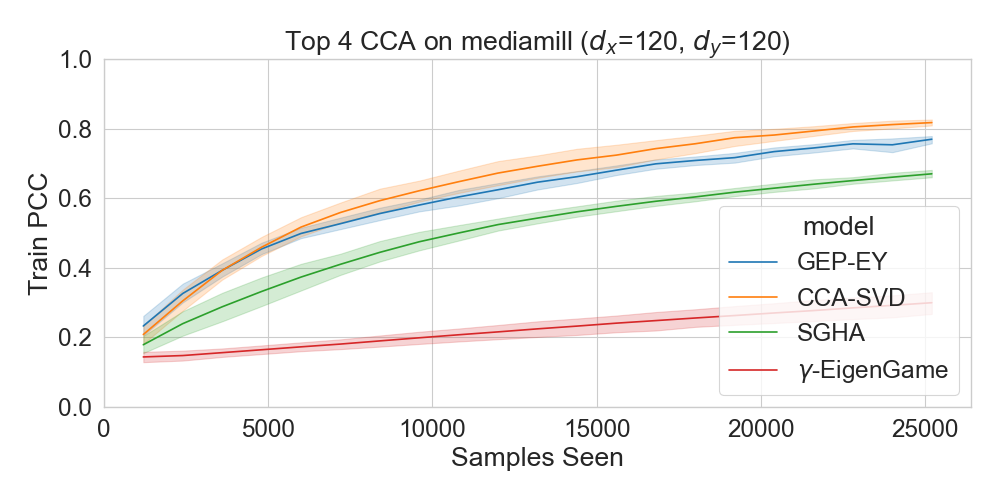
\includegraphics[width=\textwidth]{figures/gradient_descent/CCA/mediamill_100_pcc_lr_tuned.png}
        \label{fig:ccamediamill}
    \end{subfigure}
    \hfill
    \begin{subfigure}[b]{0.49\textwidth}
        \centering
        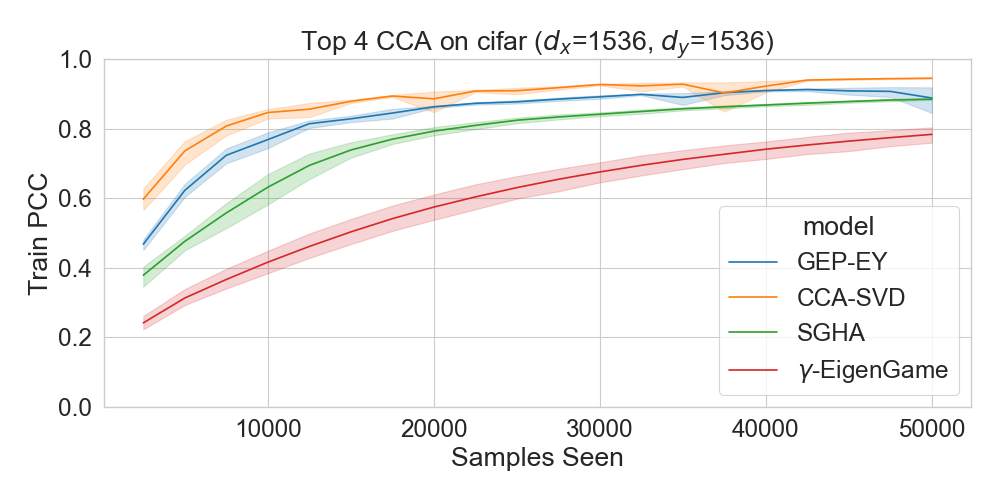
\includegraphics[width=\textwidth]{figures/gradient_descent/CCA/cifar_100_pcc_lr_tuned.png}
        \label{fig:ccacifar}
    \end{subfigure}
    \caption{PCC with respect to Scipy ground truth by GEP-EY and CCA-SVD vs prior work for (a) MediaMill and (b) Split CIFAR data. The maximum value is 1.0 and shading represents $\pm$ 1 standard deviation.}
    \label{fig:ccaiter}
    \label{fig: stochasticcca}
\end{figure}

\subsubsection{Stochastic CCA Minibatch Size}
In this section, we take a closer look at how minibatch sizes impact the performance of our method in the stochastic CCA setting. We maintain a constraint of single epoch training. This means that when we use smaller minibatches, the number of training steps increases correspondingly.

Our experiments, as displayed in Figure~\ref{fig:minibatch size ablation}, show that our method performs well across a range of minibatch sizes. Notably, it achieves high performance even when the minibatch size is nearly equivalent to the number of components.

This indicates that our method can learn effectively from a limited number of samples. It suggests the possibility of applying our method to analyse large datasets on devices with restricted memory, by processing small minibatches of data sequentially. This robustness to minibatch size could potentially make our method a viable solution for large-scale data analysis where computational resources are limited.

\begin{figure}[h]
    \centering
    \begin{subfigure}[b]{0.49\textwidth}
        \centering
        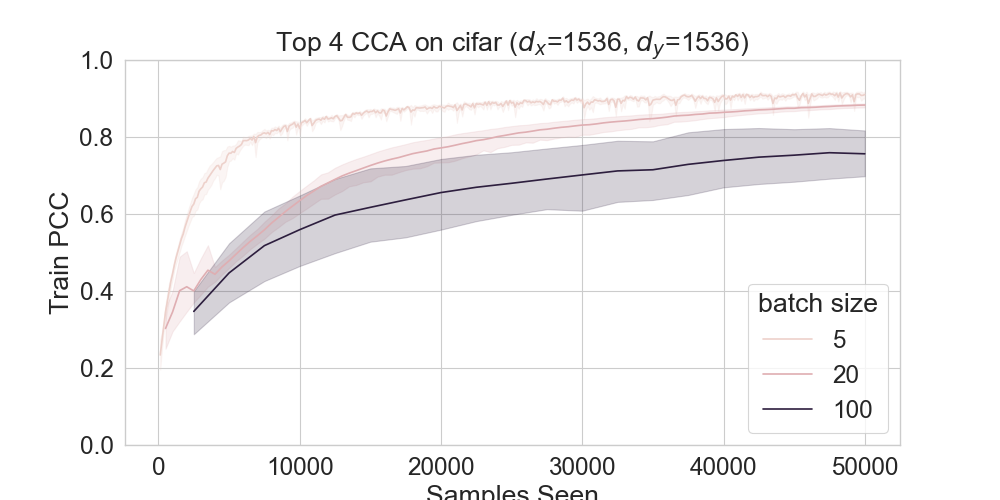
\includegraphics[width=\textwidth]{figures/gradient_descent/CCA/cifar_minibatch_size_ablation.png}
        \caption{}
        \label{fig:cifar_minibatch_ablation}
    \end{subfigure}
    \begin{subfigure}[b]{0.49\textwidth}
        \centering
        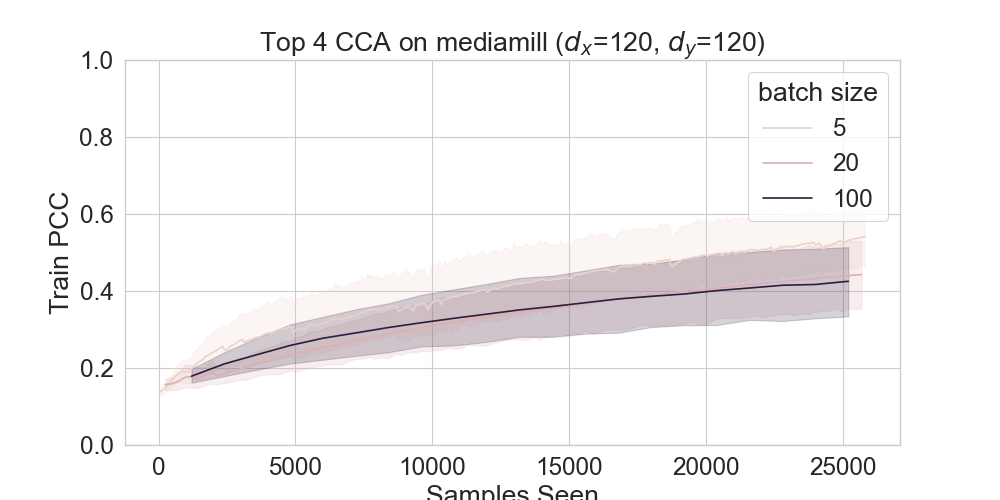
\includegraphics[width=\textwidth]{figures/gradient_descent/CCA/mediamill_minibatch_size_ablation.png}
        \caption{}
        \label{fig:mediamill_minibatch_ablation}
    \end{subfigure}
    \caption{Ablation study on minibatch size for stochastic CCA for (a) cifar and (b) mediamill datasets for minibatch sizes 100, 20, and 5}
    \label{fig:minibatch size ablation}
\end{figure}

\subsection{Discussion}



%Stochastic PLS UKBB
%%%%%%%%%%%%%%%%%%%%%%%%%%%%%%%%%%%%%%%%%%%%%%%%%%%%%%%%%%%%%%%%%%%%%%%%%%%%%%%%%%%%%%
\section{Experiment 2: Application of PLS-EY to PLS on large scale biomedical data}

\subsection{Experiment Design}

\subsection{Data}
\textbf{The UK Biobank}: is arguably the largest scale biomedical database in the world with around half a
million
total participants. The goal is to have imaging data for the brain, heart, and body for 100,000 participants. The UK Biobank combines these images with genetics, biomarkers, electronic health record, and online questionnaires making it a rich dataset for broad studies of health.

For the GEP-EY PLS analysis on biomedical data, we used 33,333 subjects from the UK Biobank \citep{sudlow2015uk}. We used pre-processed (using FreeSurfer \citep{Fischl2012}) grey-matter volumes for 66 cortical (Desikan-Killiany atlas) and 16 subcortical brain regions and 582,565 autosomal genetic variants. The affects of age, age squared, intracranial volume, sex, and the first 20 genetic principal components for population structure were removed from the brain features using linear regression to account for any confounding effects. Each brain ROI was normalised by removing the mean and dividing the standard deviation. We processed the genetics data using PLINK \citep{Purcell2007} keeping genetic variants with a minor allele frequency of at least 1\%  and a maximum missingness rate of 2\%. We used mean imputation to fill in missing values and centered each variant.

To generate measures of genetic disease risk, we calculated polygenic risk scores using PRSice \citep{PRSice2014}. We calculated scores, with a p-value threshold of 0.05, using GWAS summary statistics for the following diseases; Alzheimer's \citep{Lambert2013}, Schizophrenia \citep{Trubetskoy2022}, Bipolar \citep{Mullins2021}, ADHD \citep{Demontis2023}, ALS \citep{Van_Rheenen2021}, Parkinson's \citep{Nalls2019}, and Epilepsy \citep{International_League_Against_Epilepsy_Consortium_on_Complex_Epilepsies2018}, using the referenced GWAS studies.

We demonstrate the power of GEP-EY for large-scale subspace learning by solving PLS on imaging genetics data from the UK Biobank \citep{sudlow2015uk}, a biomedical database.
This can reveal novel phenotypes of interest and uncover genetic mechanisms of disease and brain morphometry.
Previous imaging genetics analyses using PLS and CCA were limited to small-scale datasets \citep{Lorenzi2018,Taquet2021,Lefloch2012}, which are prone to overfitting and instability.
Full batch approaches are infeasible for this data due to the high computational cost.
The only other large-scale PLS analysis on the UK Biobank used a federated approach with local batch PLS-SVD \citep{lorenzi2016}, which approximates the global solution.
We present the first stochastic PLS analysis on large-scale biomedical data.

We ran GEP-EY with minibatch size 500 on brain imaging (82 regional volumes) and genetics (582,565 variants) data for 33,333 subjects; a massive amount of data that challenges existing methods.
See supplement (Section~\ref{sec:ukbb_preprocessing}) for data pre-processing details.
We see strong validation correlation between all 10 corresponding pairs of vectors in the PLS subspace and weak cross correlation, indicating that our model learnt a coherent and orthogonal subspace of covariation (Figure~\ref{fig:UKBB_corr}), a remarkable feat for such high-dimensional data.
We found that the PLS brain subspace was associated with genetic risk measures for several disorders (Figure~\ref{fig:genetic_risk}), suggesting that the PLS subspace encodes relevant information for genetic disease risk, a significant finding for biomedical research.


% First Figure
\begin{figure}
    \centering
    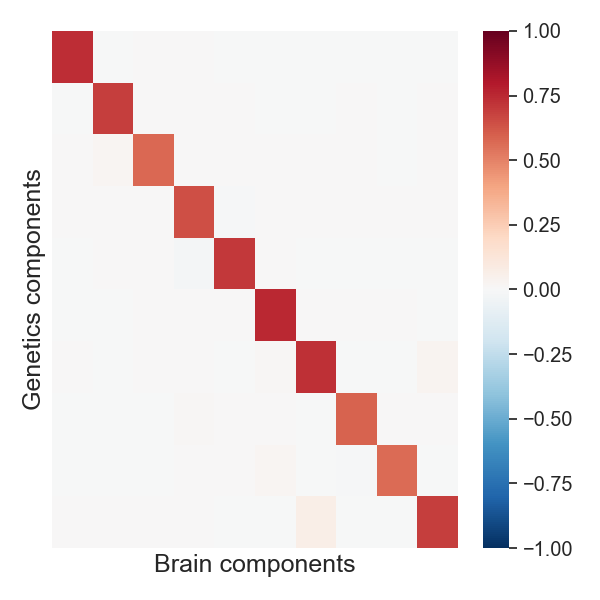
\includegraphics[width=0.5\textwidth,trim={0.8cm 0cm 0.3cm 0cm}]{figures/gradient_descent/UKBB/cross_corr}
    \caption{Correlations between PLS components for UK Biobank. This figure shows strong validation correlation between all 10 corresponding pairs of vectors in the PLS subspace and weak cross correlation, demonstrating that our model has learned a coherent and orthogonal subspace of covariation.}
    \label{fig:UKBB_corr}
\end{figure}

% Second Figure
\begin{figure}
    \centering
    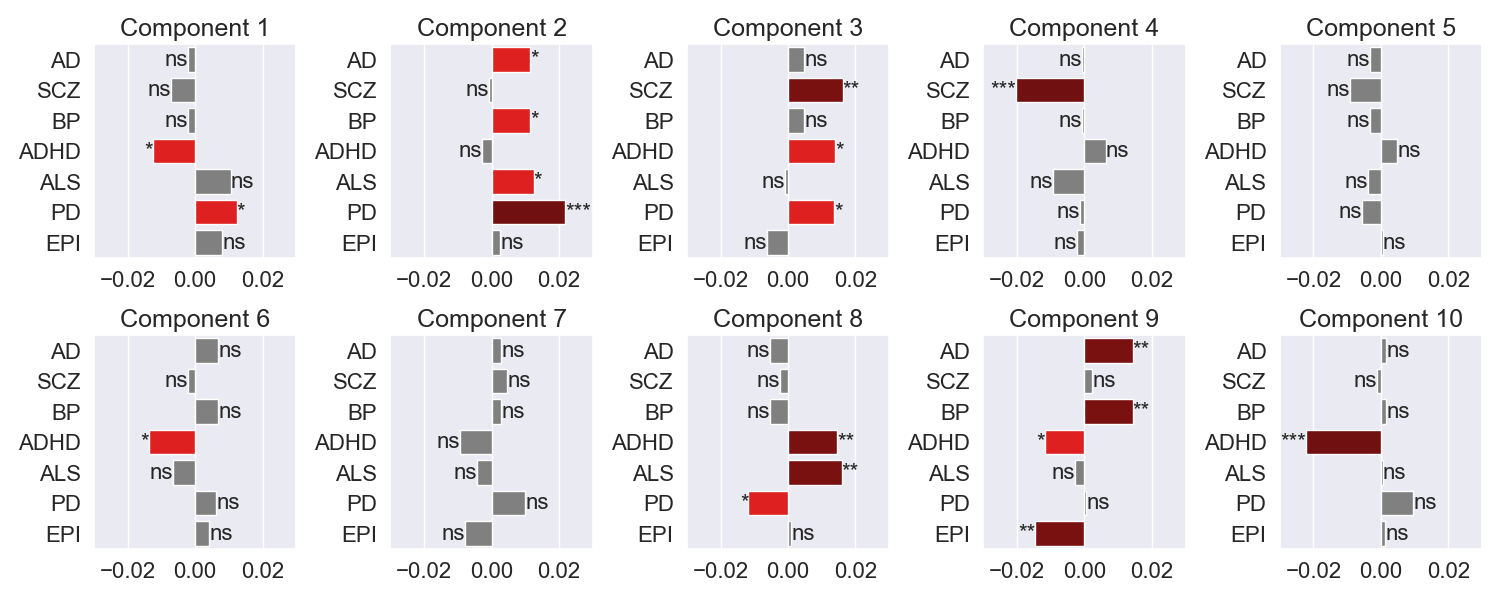
\includegraphics[width=0.7\textwidth,trim={0.5cm 0cm 0.7cm 0cm}]{figures/gradient_descent/UKBB/prs_correlations}
    \caption{Correlations between PLS brain components and genetic risk scores for several disorders. AD=Alzheimer's disease, SCZ=Schizophrenia, BP=Bipolar, ADHD=Attention deficit hyperactivity disorder, ALS=Amyotrophic lateral sclerosis, PD=Parkinson's disease, EPI=Epilepsy. The p-value significance levels are indicated as $\text{ns}: 0.05< p <= 1, \ast: 0.01< p <=0.05, \ast\ast: 0.001< p <= 0.01, \ast\ast\ast: 0.0001< p <= 0.001$. This suggests that the PLS subspace encodes relevant information for assessing genetic disease risk, an important contribution to biomedical research.}
    \label{fig:genetic_risk}
\end{figure}


\subsection{Discussion and Conclusion}

\section{Conclusion}

We presented a new unconstrained objective to characterise GEPs; this immediately gave efficient algorithms to solve many subspace learning methods in the stochastic setting with SGD.
Crucially, the gradient estimates are unbiased and cheap to compute.
Moreover, the only hyperparameter is the choice of optimiser.
We will later show how this work can be adapted and applied to optimise regularised GEPs and, in particular, CCA.

\appendix

\section{Appendix}